\documentclass[10pt,landscape]{article}
\usepackage{multicol,multirow}
\usepackage{calc}
\usepackage{ifthen}
\usepackage[landscape]{geometry}
\usepackage[colorlinks=true,citecolor=blue,linkcolor=blue]{hyperref}
\usepackage[fleqn]{amsmath}
\usepackage{amssymb,amsthm,amsfonts}
\usepackage{graphicx}

\ifthenelse{\lengthtest { \paperwidth = 11in}}
    { \geometry{top=.3in,left=.3in,right=.3in,bottom=.3in} }
	{\ifthenelse{ \lengthtest{ \paperwidth = 297mm}}
		{\geometry{top=1cm,left=1cm,right=1cm,bottom=1cm} }
		{\geometry{top=1cm,left=1cm,right=1cm,bottom=1cm} }
	}
\pagestyle{empty}
\makeatletter
\renewcommand{\section}{\@startsection{section}{1}{0mm}%
                                {-1ex plus -.5ex minus -.2ex}%
                                {0.5ex plus .2ex}%x
                                {\normalfont\large\bfseries}}
\renewcommand{\subsection}{\@startsection{subsection}{2}{0mm}%
                                {-1explus -.5ex minus -.2ex}%
                                {0.5ex plus .2ex}%
                                {\normalfont\normalsize\bfseries}}
\renewcommand{\subsubsection}{\@startsection{subsubsection}{3}{0mm}%
                                {-1ex plus -.5ex minus -.2ex}%
                                {1ex plus .2ex}%
                                {\normalfont\small\bfseries}}
\renewcommand{\arraystretch}{1.3}
\makeatother
\setcounter{secnumdepth}{0}
\setlength{\parindent}{0pt}
\setlength{\parskip}{0pt plus 0.5ex}
\setlength{\mathindent}{0pt}
% -----------------------------------------------------------------------

\title{Partial Differential Equations}

\begin{document}

\raggedright
\footnotesize

\begin{center}
     \textbf{Partial Differential Equations} \\
\end{center}
\begin{multicols}{3}
\setlength{\premulticols}{1pt}
\setlength{\postmulticols}{1pt}
\setlength{\multicolsep}{1pt}
\setlength{\columnsep}{2pt}

\section{Derivatives}
\begin{tabular}{r|l}
	$f(x)$ & $\frac{df}{dx}$ \\
	\hline
	$\sinh(x)$ & $\cosh(x)$ \\
	$\cosh(x)$ & $\sinh(x)$ \\
	$\mathrm{arcsinh}(x)$ & $1 \div \sqrt{x^2+1}$ \\
	$\mathrm{arccosh}(x)$ & $1 \div \sqrt{x^2 - 1}$ ($1<x$)
\end{tabular}

\section{Integrals}
\begin{tabular}[h]{rl}
	$\int x^n\ dx$ & $= \frac{1}{n+1}x^{n+1} + C$ \\
	$\int \frac{1}{x}\ dx$ & $= \ln |x| + C$ \\
	$\int \frac{1}{ax + b}\ dx$ & = $\frac{1}{a} \ln |ax+b| + C$ \\
	$\int \frac{1}{(x+a)^2}\ dx$ & $= -\frac{1}{x+a} + C$ \\
	$\int \frac{1}{1 + x^2}$ & $= \tan^{-1} x + C$ \\
	$\int \ln ax\ dx$ & $= x\ln ax - x + C$ \\
	$\int e^{ax}\ dx$ & $= \frac{1}{a} e^{ax} + C$ \\
	$\int \sin(ax)\ dx$ & $= -\frac{1}{a}\cos(ax) + C$ \\
	$\int \sin^2(ax)\ dx$ & $= \frac{x}{2}-\frac{\sin(2ax)}{4a} + C$ \\
	$\int x\cos x\ dx$ & $= \cos x + x\sin x + C$ \\
	$\int \sinh(ax)\ dx$ & $= a^{-1}\cosh{ax} + C$ \\
	$\int \cosh(ax)\ dx$ & $= a^{-1}\sinh{ax} + C$ \\
\end{tabular}

\section{Integration Techniques}
\subsubsection{Integration by Parts}
\begin{equation*}
	\int_a^b u(x)v'(x)\ dx = \left[ u(x)v(x) \right]_a^b-\int_a^bu'(x)v(x)\ dx
\end{equation*}

Or, with $u=u(x)$, $du=u'(x)\ dx$, $v=v(x)$ and $dv=v'(x)\ dx$:
\begin{equation*}
	\int u\ dv=uv - \int v\ du
\end{equation*}

\subsubsection{Substitution}
\begin{equation*}
	\int_a^b f(g(x))\cdot g'(x)\ dx = \int_{g(a)}^{g(b)}f(u)\ du
\end{equation*}

\subsubsection{Leibniz integral rule}
\begin{multline*}
	\frac{d}{dx}\left(\int_{a(x)}^{b(x)}f(x,t)\ dt\right)
	=
	\\
	f(x,b(x))\cdot\frac{d}{dx}b(x)
	-f(x,a(x))\cdot\frac{d}{dx}a(x)
	+\int_{a(x)}^{b(x)}\frac{\partial}{\partial x}f(x,t)\ dt
\end{multline*}
Special case where $a(x)=a=\mathrm{const.}$ and $b(x)=b=\mathrm{const.}$:
\begin{equation*}
	\frac{d}{dx}\left(\int_a^b f(x,t)\ dt\right)
	=\int_a^b\frac{\partial}{\partial x}f(x,t)\ dt
\end{equation*}

\section{Domain and Boundary}
\begin{itemize}
	\item Domain $\Omega$ is an open subset of $\mathbb{R}^n$ (meaning all points are interior points)
	\item Boundary has to meet conditions:
	\item{ \emph{Dirichlet boundary conditions}: specify values $u$ on $\partial\Omega$: \\
		$u(x) = f(x)\ \forall x\in\partial\Omega$
	}
	\item{\emph{Neumann boundary conditions}: specify derivatives of $u$ on boundary.
		Only derivatives orthogonal to the boundary give additional information: \\
		normal derivative: $\frac{\partial u}{\partial n} = g(x)\ \forall x\in\partial\Omega$
	}
\end{itemize}

\section{Classification}
\begin{center}
  \makebox[\columnwidth]{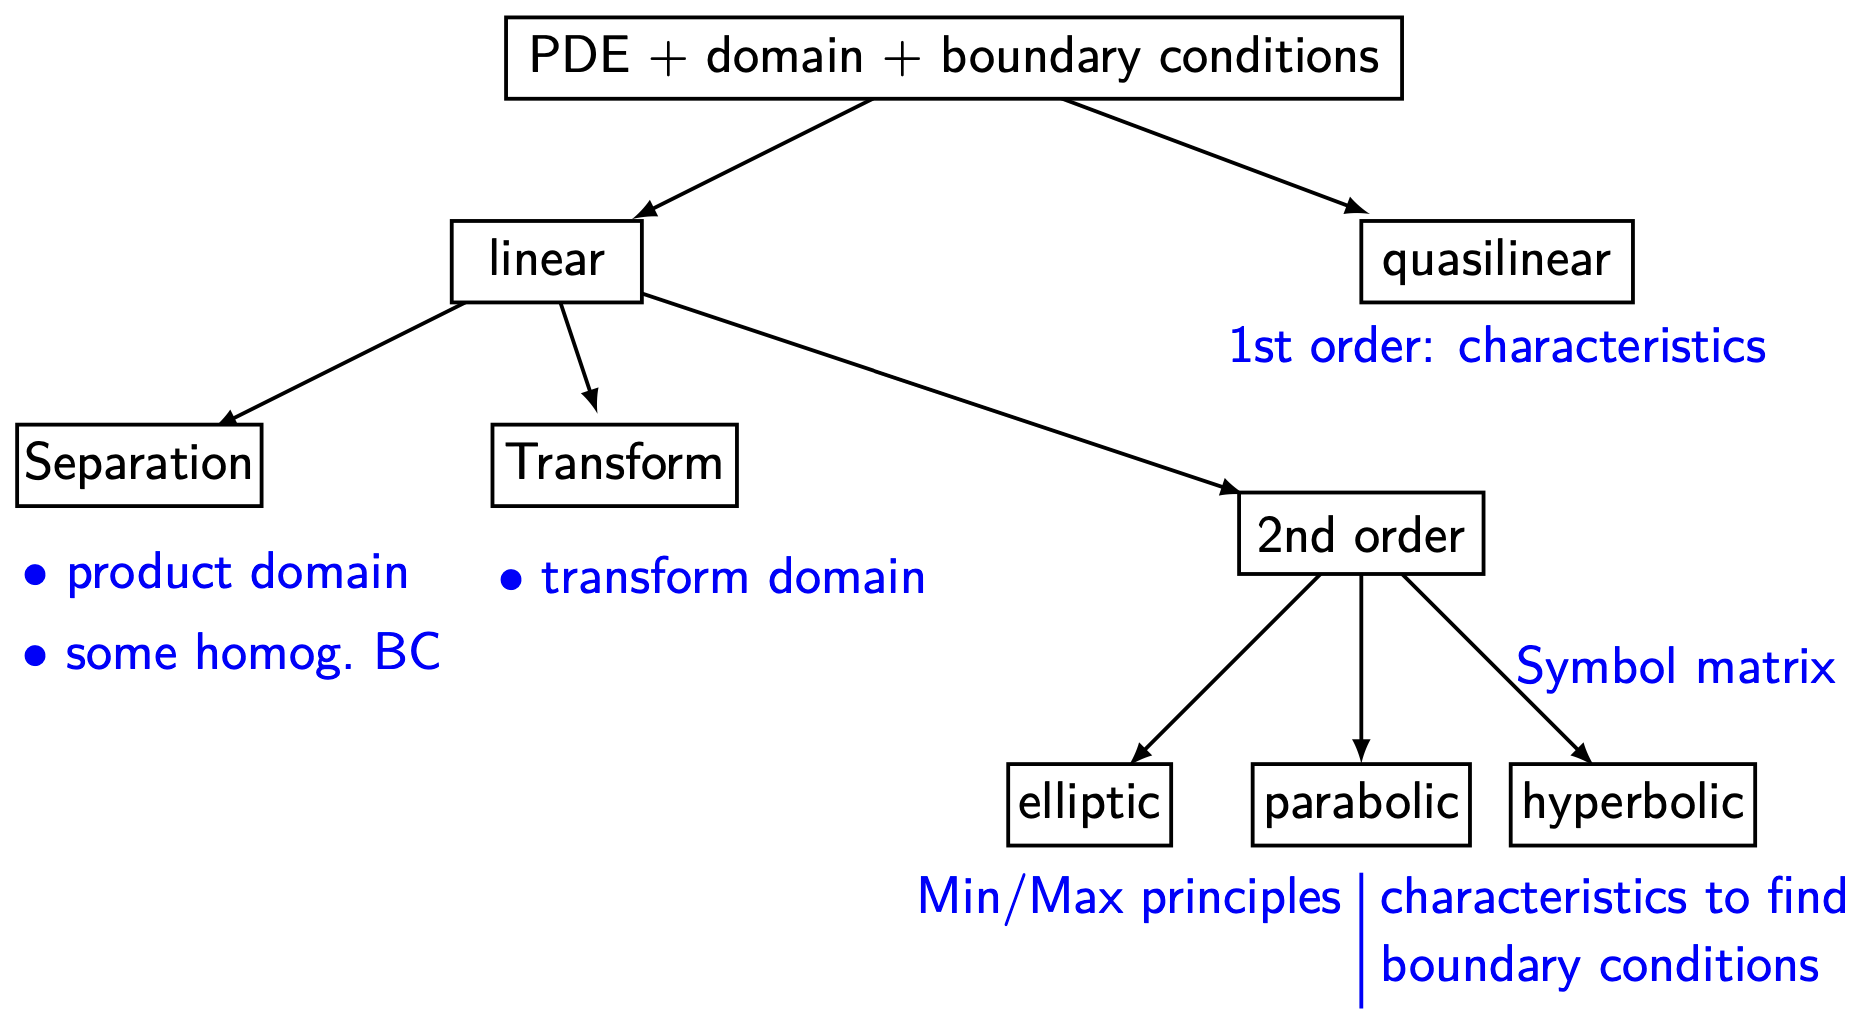
\includegraphics[width=0.9\columnwidth]{images/decision-tree}}
\end{center}

\subsection{Linearity}
Given an equation involving function $u(x), x\in\mathbb{R}$ and its derivatives,
there is a function $F$ describing the relation:
\begin{align*}
	F\left(
	\begin{matrix}
		x,y,z,p,q,s,t,r,\ldots \\
		\downarrow \text{(corresponding to)}\downarrow \\
		x, y, u, \frac{\partial u}{\partial x}, \frac{\partial u}{\partial y}, \frac{\partial^2 u}{\partial x^2},
		\frac{\partial^2 u}{\partial x\partial y},\frac{\partial^2 u}{\partial y^2}, \ldots
	\end{matrix}
	\right) = 0
\end{align*}
(common variable names $p_i\rightarrow\frac{\partial u}{\partial x_i}$ and
$t_{ij} \rightarrow\frac{\partial^2 u}{\partial x_i\partial x_j}$)

A PDE is \emph{linear} when function $F$ is linear in $u,p_1,\ldots,p_n,t_{11},\ldots,t_{nn},\ldots.$

A PDF is \emph{quasilinear} when function $F$ is linear in $p_1,\ldots,p_n,t_{11},\ldots,t_{nn},\ldots.$

For example, given the heat equation $u_t=\kappa u_{xx}$, $F$ would be $F(p_1,t_{22})=p_1-\kappa t_{22}$.

\subsection{2\textsuperscript{nd} Order PDEs: Symbol Matrix}

The symbol matrix of the 2\textsuperscript{nd} order partial differential operator

\begin{align*}
	L=\sum_{i,j=1}^{n}a_{ij}(x)\frac{\partial^2}{\partial x_i \partial x_j}+\sum_{i=1}^n b_i(x)\frac{\partial}{\partial x_i}+c(x)
\end{align*}

is the symmetric matrix

\begin{align*}
	A=
	\begin{bmatrix}
		a_{11} & a_{12} & \ldots & a_{1n} \\
		a_{21} & a_{22} & \ldots & a_{2n} \\
		\vdots & \vdots & \ddots & \vdots \\
		a_{n1} & a_{n2} & \ldots & a_{nn}
	\end{bmatrix}
\end{align*}

For example:

\begin{center}
  \makebox[\columnwidth]{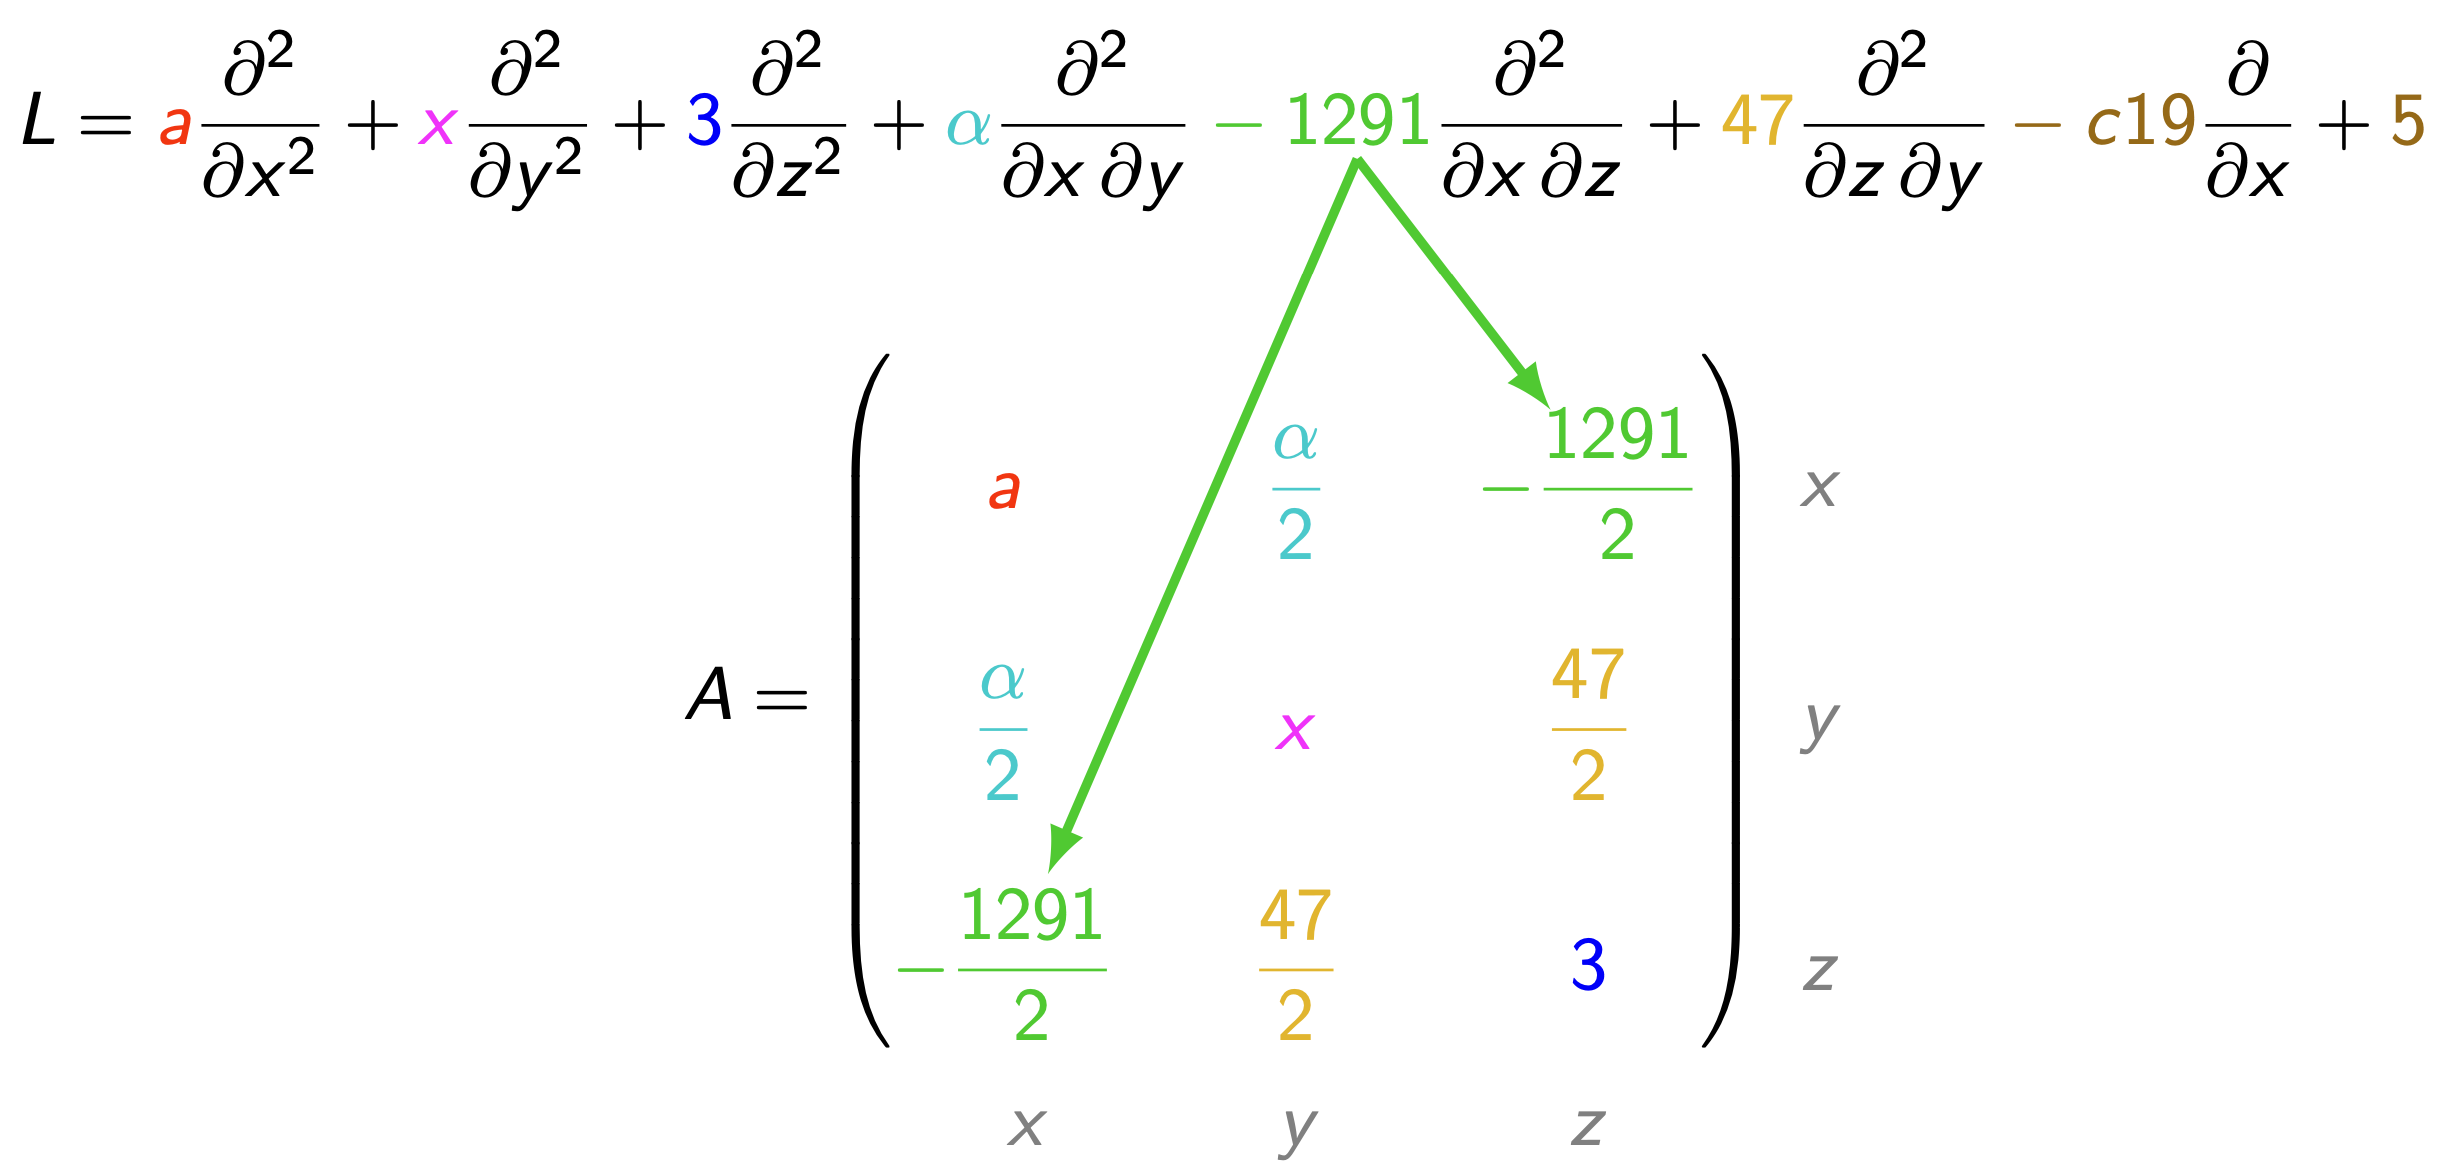
\includegraphics[width=0.9\columnwidth]{images/symbol-matrix}}
\end{center}

The type of equation can be inferred by the sign of the eigenvalues $\lambda_1,\ldots,\lambda_n$ of the symbol matrix. 
Calculating the determinant ($\det A=\prod_i \lambda_i$) and trace ($\mathrm{tr}\ A=\sum_i \lambda_i$)
reveals information about the signs of its eigenvalues:

\begin{center}
  \makebox[\columnwidth]{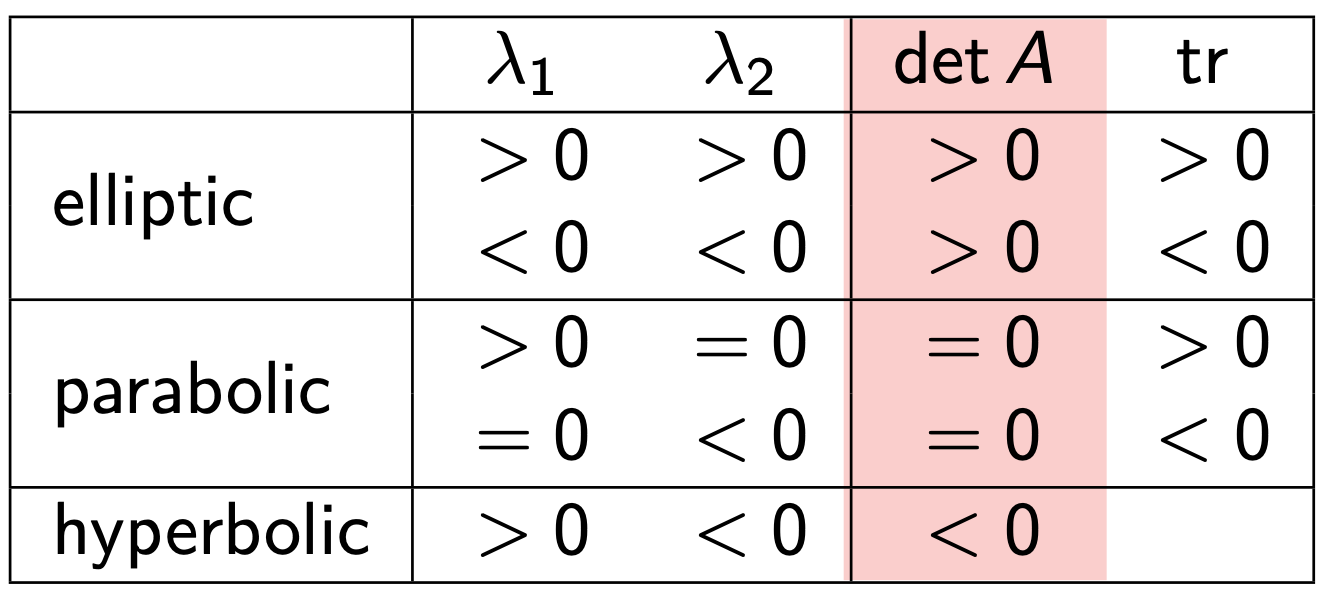
\includegraphics[width=0.5\columnwidth]{images/classification}}
\end{center}

\section{Quasilinear PDEs}

Given a PDE $F(x,y,u,\frac{\partial u}{\partial x},\frac{\partial u}{\partial y}) = 0$, the PDE defines a relation between the two slopes: $F(x,y,u,m_x,m_y)=0$

\subsection{Characteristics}

The PDE

\begin{align*}
	a(x,y,u)\frac{\partial u}{\partial x}+b(x,y,u)\frac{\partial u}{\partial y} - c(x,y,u) = 0
\end{align*}
can be written in vector notation:
\begin{align*}
  {\color{red}
    \underbrace{
      \begin{pmatrix}
        a(x,y,u) \\
        b(x,y,u) \\
        c(x,y,u)
      \end{pmatrix}
    }_{\vec t}
  }
  \cdot
  {\color{blue}
    \begin{pmatrix}
      \frac{\partial u}{\partial x}\\
      \frac{\partial u}{\partial y}\\
      -1
    \end{pmatrix}
  }
  &= 0
\end{align*}

\section{Numerical Methods}
\subsection{Discretisation of Operators}

\begin{align*}
	\frac{\partial g}{\partial x}
	\approx
	\frac{g(x + \Delta x) - g(x)}{\Delta x}
\end{align*}

\begin{align*}
	\frac{\partial^2 g}{\partial x^2}
	\approx
	\frac{g(x + \Delta x) - 2\cdot g(x) + g(x - \Delta x)}{\Delta x^2}
\end{align*}

($\Delta$ referring to step size)
\subsection{Finite Elements}

We have a set of given local basis functions $v_1(x), \ldots, v_n(x)$ that are continuous and piecewise differentiable.
We subdivide $\Omega$ into meshes and assign each nodal point a nodal variable $a_k$.
Then, we use shape functions to represent the PDE on the mesh,
e.g. using triangular functions $l_1(x)=1-x$ and $l_2(x) = x$ to obtain \emph{local} element matrices
\begin{align*}
	E = 
	\begin{bmatrix}
		\int_0^1 l_1^\prime(s)\cdot l_1^\prime(s)\ ds & \int_0^1 l_1^\prime(s)\cdot l_2^\prime(s)\ ds \\
		\int_0^1 l_2^\prime(s)\cdot l_1^\prime(s)\ ds & \int_0^1 l_2^\prime(s)\cdot l_2^\prime(s)\ ds
	\end{bmatrix}
	=
	\begin{bmatrix}
		1 & -1 \\
		-1 & 1
	\end{bmatrix}
\end{align*}

that can then be used to construct the mesh matrix $M=1/h\cdot E$ using mesh size $h$.
Afterwards, the global Ritz matrix can be computed, e.g. for a one-dimensional mesh with 4 nodal points and 2 unknown inner points,
yielding 4 base functions $v_1,v_2,v_3,v_4$:

\begin{align*}
	R^4 = \begin{bmatrix}
		{\color{red} M^{(1)}_{0,0}} & \color{red}{M^{(1)}_{0,1}} & 0 & 0 \\
		{\color{red} M^{(1)}_{1,0}} & {\color{red} M^{(1)}_{1,1}} + {\color{blue} M^{(2)}_{0,0}} & {\color{blue} M^{(2)}_{0,1}} & 0 \\
		0 & {\color{blue} M^{(2)}_{1,0}} & {\color{blue} M^{(2)}_{1,1}} + {\color{green} M^{(3)}_{0,0}} & {\color{green} M^{(3)}_{0,1}} \\
		0 & 0 & {\color{green} M^{(3)}_{1,0}} & {\color{green} M^{(3)}_{1,1}}
	\end{bmatrix}
\end{align*}

The system vector can then be calculated:

\begin{align*}
	\vec{r^4} = \begin{pmatrix}
		\int_0^1 f(x)\cdot v_0(x)\ dx \\
		\vdots \\
		\int_0^1 f(x)\cdot v_3(x)\ dx
	\end{pmatrix}
\end{align*}

Finally, we have obtained the Ritz system: $R^4\cdot\vec{a}=\vec{r^4}$.
That yields the approximation function (as defined by the ansatz): $\tilde{u}(x)=\sum_{i=0}^3 a_i\cdot v_i(x)$
3with $a_0$ and $a_3$ fulfilling the boundary conditions.

\end{multicols}

\end{document}
